\documentclass[../structural_economics_book.tex]{subfiles}
\begin{document}
\ifSubfilesClassLoaded{\setcounter{chapter}{5}}{}
\chapter{Centrality, Power, and the Perron Vector}\label{ch:06}
\chaptersubtitle{Where Power Comes From}
% TODO-VERIFY: locate this sentence in Prebisch, Capitalismo Periferico (Mexico: FCE, 1981) and add a page number; it may be a paraphrase.
\begin{quote}
\textit{``En el capitalismo perif\'{e}rico, la apropiaci\'{o}n del excedente econ\'{o}mico est\'{a} \'{i}ntimamente ligada a las relaciones de poder entre los distintos estratos sociales.''}\\[0.3em]
\textnormal{[``In peripheral capitalism, the appropriation of the economic surplus is intimately linked to the power relations between different social strata.'']}\\
\hfill --- Ra\'{u}l Prebisch, \textit{Capitalismo Perif\'{e}rico: Crisis y Transformaci\'{o}n} (1981)
\end{quote}

\vspace{0.3em}

\begin{quote}
\textit{``Power is not an institution, and not a structure; neither is it a certain strength we are endowed with; it is the name that one attributes to a complex strategical situation in a particular society.''}\\
\hfill --- Michel Foucault, \textit{The History of Sexuality} (1976)
\end{quote}

\vspace{0.5em}

\begin{quote}
\textit{``Power is the left Perron eigenvector of the weight matrix.''}\\
\hfill --- This book
\end{quote}

\vspace{1em}

Foucault insisted that power is relational, not an attribute of individuals. This chapter takes that relational view and asks how much of it can be measured. Our answer is partial but precise: one dimension of power is a property of the network --- specifically, of the row-stochastic weight matrix $W$ that encodes who affects whom (Chapter~1, Section~\ref{ch01:sec:conventions}). It is computed from the Perron-Frobenius theorem.

This chapter does three things. First, it develops the concept of centrality --- the idea that some positions in a network are more ``important'' than others --- through examples, building from simple degree counting to the recursive logic of eigenvector centrality. Second, it states and proves the Perron-Frobenius theorem, which guarantees that the centrality measure we want actually exists and is unique. Third, it derives the properties of the Perron eigenvector --- the power vector $\boldsymbol{\pi}$ --- and separates two things the spectral gap $\Gamma$ is often taken to measure: the \textit{integration} of the network (which $\Gamma$ does measure) and the \textit{concentration} of power (which it does not; that is measured by $\Neff$ and $\Var(\pi)$).

By the end, the student will know where power comes from (the network), how to compute it (the Perron eigenvector), how to measure its concentration (the effective number of agents $\Neff$), why the spectral gap is a separate coordinate (Proposition~\ref{ch06:prop:gap-power-independent}), and when power is equal ($W$ doubly stochastic) --- a distributional condition, not an efficiency condition.


%% =====================================================================
\section{Who Matters? Four Attempts at an Answer}
\label{ch06:sec:who_matters}
%% =====================================================================

\subsection{A Small Economy}

Consider five agents in a production network. Following the book's convention, $W$ is row-stochastic: row $i$ is the distribution of agent $i$'s dependence (input-cost shares, $W^P = D^{-1}A$ in the notation of Chapter~1), so each row sums to one. \illustrative

\begin{equation}\label{ch06:eq:W5}
W = \begin{pmatrix}
0.4 & 0.4 & 0.1 & 0.1 & 0.0 \\
0.3 & 0.3 & 0.2 & 0.2 & 0.0 \\
0.1 & 0.2 & 0.3 & 0.2 & 0.2 \\
0.0 & 0.1 & 0.4 & 0.3 & 0.2 \\
0.0 & 0.1 & 0.1 & 0.3 & 0.5
\end{pmatrix}.
\end{equation}

Read row $i$: these are the weights that agent $i$ places on others. Agent 1 depends heavily on agent 2 ($W_{12} = 0.4$). Agent 5 depends heavily on herself ($W_{55} = 0.5$) and on agent 4 ($W_{54} = 0.3$). Agent 3 is in the middle --- connected to everyone.

Question: which agent is the most powerful?

Four different answers emerge from four different ways of measuring importance. All four are ``correct'' in their own domain. Only one is the right measure of structural power.


\subsection{Attempt 1: Count the Connections (Degree Centrality)}

The simplest measure: how many connections does each agent have?

\begin{definition}[Degree Centrality]\label{ch06:def:degree}
For a weight matrix $W$, agent $i$'s \textbf{in-degree} is the column sum $d_i^{\text{in}} = \sum_{j} W_{ji}$ (total weight that others place on $i$). The \textbf{out-degree} is the row sum $d_i^{\text{out}} = \sum_j W_{ij}$ (total weight that $i$ places on others).
\end{definition}

For our $W$: the column sums (in-degree) are:

\begin{center}
\begin{tabular}{lccccc}
\toprule
Agent & 1 & 2 & 3 & 4 & 5 \\
\midrule
In-degree $d^{\text{in}}_i$ & 0.80 & 1.10 & 1.10 & 1.10 & 0.90 \\
\bottomrule
\end{tabular}
\end{center}

Agents 2, 3 and 4 are tied at the top: each receives the most total weight from others. Agent 1 is least important by this measure.

\begin{intuition}[What degree gets right and wrong]
Degree counts \textit{direct} connections: how many people depend on you (in-degree) or how much you depend on others (out-degree). It is easy to compute and often correlates with importance. But it misses something critical: \textit{who} depends on you matters. If you are depended upon by powerful agents, that should count more than being depended upon by peripheral agents. Degree treats all connections equally. A farmer who sells to the president and a farmer who sells to another farmer have the same in-degree, but they do not have the same power.
\end{intuition}


\subsection{Attempt 2: Count the Paths (Katz Centrality)}

Degree counts direct connections. A more sophisticated measure counts \textit{all} paths --- direct and indirect.

\begin{definition}[Katz Centrality]\label{ch06:def:katz}
Agent $i$'s \textbf{Katz centrality} is:
\begin{equation}\label{ch06:eq:katz}
c_i^{\text{Katz}} = \sum_{k=1}^{\infty} \delta^k \sum_{j=1}^N (W^k)_{ji} = \left[(I - \delta W')^{-1} - I\right]_{i} \cdot \ones,
\end{equation}
where $\delta \in (0, 1/\rho(W))$ is a decay parameter that downweights longer paths ($\rho(W) = 1$ for row-stochastic $W$), and $(W^k)_{ji}$ is the total weight of all paths of length $k$ from $i$ to $j$.
\end{definition}

Katz centrality says: agent $i$ is important if many paths lead to her, directly or indirectly, weighted by length. The parameter $\delta$ ensures convergence of the Neumann series.

\begin{intuition}[The Leontief connection]
In matrix form, $\mathbf{c}^{\text{Katz}}$ is the vector of column sums of $(I - \delta W)^{-1}$, minus one. This is the same Neumann series as the Leontief inverse of Chapter~1 --- but there it is applied to the technical-coefficient matrix $A$, which is what output multipliers require. Applied to a row-stochastic $W$, it is a centrality measure, not a multiplier (all row sums of $(I-\delta W)^{-1}$ equal $1/(1-\delta)$).

Katz improves on degree by counting indirect connections. Its limitation is the analyst-chosen $\delta$: short paths dominate when $\delta$ is small, long paths when $\delta$ is close to $1/\rho$. As $\delta \to 1/\rho$, the normalized Katz vector converges to the eigenvector centrality of Attempt~4 --- the measure that counts paths of every length without discounting.
\end{intuition}


\subsection{Attempt 3: Ask the Neighbors (Bonacich Centrality)}

\begin{definition}[Bonacich Centrality]\label{ch06:def:bonacich}
Agent $i$'s \textbf{Bonacich centrality} is the $i$-th component of:
\begin{equation}\label{ch06:eq:bonacich}
\mathbf{c}^{\text{Bon}} = (I - \beta W')^{-1} W' \ones = (I - \beta W')^{-1} \mathbf{d}^{\text{in}},
\end{equation}
where $\beta \in (-1/\rho(W), 1/\rho(W))$ is a parameter and $\mathbf{d}^{\text{in}} = W'\ones$ is the in-degree vector.
\end{definition}

Bonacich centrality starts from degree (the $\mathbf{d}^{\text{in}}$ term) and then amplifies it through the Leontief-type multiplier $(I - \beta W')^{-1}$. As defined here it is Katz centrality rescaled: since $(I-\beta W')^{-1}\beta W' = (I-\beta W')^{-1} - I$,
\begin{equation}\label{ch06:eq:bonacich_katz}
\mathbf{c}^{\text{Bon}}(\beta) = \tfrac{1}{\beta}\,\mathbf{c}^{\text{Katz}}(\beta) \qquad (\beta \neq 0),
\end{equation}
so for $\beta > 0$ the two rank agents identically. Bonacich's (1987) contribution is the interpretation of the parameter, including negative values.

The parameter $\beta$ has a remarkable interpretation. When $\beta > 0$, an agent is more central if her neighbors are also central --- this captures \textit{cooperation} (your friends' power helps you). When $\beta < 0$, an agent is more central if her neighbors are \textit{less} central --- this captures \textit{bargaining} (your power comes from your partners' weakness, because they have no outside options).

Ballester, Calv\'{o}-Armengol, and Zenou (2006) proved the foundational result: in linear-quadratic games on networks, the Nash equilibrium action of each agent is proportional to her Bonacich centrality. This is the ``Bonacich-Nash linkage'' --- the first clean mapping from network position to economic outcome.

\begin{intuition}[Getting closer]
Katz and Bonacich already make the centrality of your neighbors matter, through the indirect paths. But both depend on a parameter that must be chosen by the analyst, and different values give different rankings. There is no ``canonical'' Bonacich centrality.

The eigenvector centrality of the next subsection is the limit of the normalized Katz/Bonacich vector as the parameter approaches $1/\rho(W)$. It is therefore not a different idea but the parameter-free end of the same family --- determined entirely by the network. Choosing it is a modelling decision: it is the right object for long-run (DeGroot) influence, while Katz/Bonacich are the right objects for linear-quadratic games with a finite discount.
\end{intuition}


\subsection{Attempt 4: The Recursive Definition (Eigenvector Centrality)}

Here is the idea that resolves everything.

\textit{An agent is powerful if powerful agents depend on her.}

This is circular. The power of agent $i$ depends on the power of agents $j$ who point to $i$, which depends on the power of agents $k$ who point to $j$, and so on. We seem to need to know the answer before we can compute it.

But this circularity is not a bug. It is a feature. The circularity defines a \textit{fixed-point equation}: we seek a vector $\boldsymbol{\pi}$ such that the power of each agent equals the total power directed toward her.

\begin{definition}[Eigenvector Centrality --- Left Perron Eigenvector]\label{ch06:def:eigenvector}
Agent $i$'s \textbf{eigenvector centrality} (or \textbf{structural power}) is $\pi_i$, the $i$-th component of the vector $\boldsymbol{\pi}$ satisfying:
\begin{equation}\label{ch06:eq:perron_def}
\boldsymbol{\pi}' W = \rho(W) \cdot \boldsymbol{\pi}',
\end{equation}
with $\boldsymbol{\pi} \geq 0$ and $\|\boldsymbol{\pi}\|_1 = \sum_i \pi_i = 1$. For the row-stochastic matrices used throughout this book $\rho(W) = 1$, so~\eqref{ch06:eq:perron_def} reads $\boldsymbol{\pi}'W = \boldsymbol{\pi}'$.

Equivalently, for each agent:
\begin{equation}\label{ch06:eq:perron_component}
\pi_i = \frac{1}{\rho(W)} \sum_{j=1}^N \pi_j W_{ji}.
\end{equation}
\end{definition}

\begin{intuition}[Reading the equation]
Equation~\eqref{ch06:eq:perron_component} says: agent $i$'s power is proportional to the sum, over all agents $j$, of (a) $j$'s power $\pi_j$ times (b) how much $j$ depends on $i$ (that is, $W_{ji}$). You are powerful if powerful agents point toward you.

The factor $1/\rho(W)$ is the reciprocal of the Perron eigenvalue, not a normalization (it equals one when $W$ is row-stochastic); the separate normalization $\sum_i \pi_i = 1$ fixes the scale of $\boldsymbol{\pi}$.

This is the recursive definition we wanted: power depends on the power of those who depend on you. The Perron-Frobenius theorem (next section) guarantees that this circular definition has a unique solution.
\end{intuition}

\begin{example}[Computing Power for the Five-Agent Economy]\label{ch06:ex:five_power}
For the matrix $W$ in~\eqref{ch06:eq:W5}, the left Perron eigenvector (computed iteratively --- see Appendix~6A) is:
\begin{equation}
\boldsymbol{\pi} \approx (0.144, \; 0.208, \; 0.236, \; 0.227, \; 0.185),
\end{equation}
with $\Neff = 1/\sum_i \pi_i^2 = 4.87$ (Definition~\ref{ch06:def:neff}).

\textbf{Agent 3 is the most powerful} ($\pi_3 = 0.236$), even though she tied with Agents~2 and~4 on in-degree. Why? Because Agent~3 is depended upon by Agent~4 ($W_{43} = 0.4$), who is himself powerful ($\pi_4 = 0.227$). Agent~2's largest dependent is Agent~1 ($W_{12} = 0.4$), who is the \textit{least} powerful ($\pi_1 = 0.144$). Being depended upon by a weak agent counts for less: Agent~2 falls from a tie for first on in-degree to third on eigenvector centrality.

\textbf{Agent 1 is the least powerful} ($\pi_1 = 0.144$). She is peripheral: few agents depend on her, and those who do are not particularly powerful themselves.

Compare the four centrality measures:

\begin{center}
\begin{tabular}{lccccc}
\toprule
& Agent 1 & Agent 2 & Agent 3 & Agent 4 & Agent 5 \\
\midrule
In-degree & 0.80 & \textbf{1.10} & \textbf{1.10} & \textbf{1.10} & 0.90 \\
Katz ($\delta = 0.5$) & 0.77 & 1.08 & \textbf{1.13} & 1.11 & 0.90 \\
Bonacich ($\beta = 0.3$) & 1.12 & 1.56 & \textbf{1.60} & 1.58 & 1.28 \\
Eigenvector $\pi_i$ & 0.144 & 0.208 & \textbf{0.236} & 0.227 & 0.185 \\
\bottomrule
\end{tabular}
\end{center}

Katz, Bonacich and the eigenvector agree on the ranking $3 \succ 4 \succ 2 \succ 5 \succ 1$; in-degree cannot separate Agents~2, 3 and~4. Katz and Bonacich agree exactly because of~\eqref{ch06:eq:bonacich_katz}. The eigenvector is the parameter-free limit of the family: the normalized Katz vector is $(0.152, 0.210, 0.231, 0.223, 0.185)$ at $\delta = 0.9$ and $(0.144, 0.208, 0.236, 0.227, 0.185)$ at $\delta = 0.999$.
\end{example}

\begin{vizpanel}{The five-agent economy: heatmap and power distribution}
\begin{center}
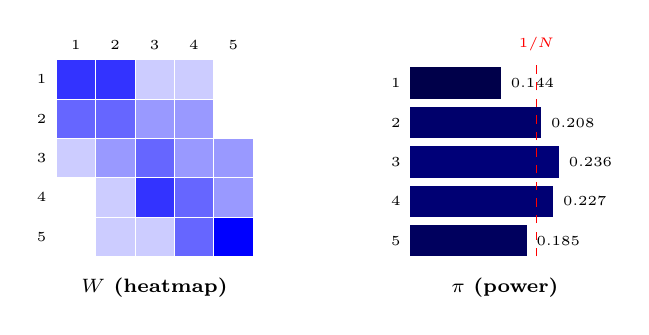
\begin{tikzpicture}[scale=1]
\def\s{0.5}
%% W heatmap (5x5), values from eq (6.1)
\foreach \i/\j/\v in {
  1/1/80,1/2/80,1/3/20,1/4/20,1/5/0,
  2/1/60,2/2/60,2/3/40,2/4/40,2/5/0,
  3/1/20,3/2/40,3/3/60,3/4/40,3/5/40,
  4/1/0,4/2/20,4/3/80,4/4/60,4/5/40,
  5/1/0,5/2/20,5/3/20,5/4/60,5/5/100} {
  \fill[blue!\v, draw=white, line width=0.15pt]
    ({(\j-1)*\s}, {(5-\i)*\s}) rectangle +(\s,\s);
}
%% Row/col labels
\foreach \k/\lab in {1/1,2/2,3/3,4/4,5/5} {
  \node[font=\tiny, left] at (0, {(5-\k+0.5)*\s}) {\lab};
  \node[font=\tiny, above] at ({(\k-0.5)*\s}, {5*\s}) {\lab};
}
\node[below, font=\scriptsize\bfseries] at ({2.5*\s}, -0.15) {$W$ (heatmap)};

%% Power bars
\begin{scope}[xshift=4.5cm]
\foreach \k/\val/\pct in {1/0.144/29,2/0.208/42,3/0.236/47,4/0.227/45,5/0.185/37} {
  \fill[blue!\pct!black] (0, {(5-\k)*0.5}) rectangle ({\val*8}, {(5-\k)*0.5+0.4});
  \node[font=\tiny, left] at (0, {(5-\k)*0.5+0.2}) {\k};
  \node[font=\tiny, right] at ({\val*8}, {(5-\k)*0.5+0.2}) {\val};
}
%% 1/N reference line
\draw[red, dashed, thin] ({0.2*8}, 0) -- ({0.2*8}, 2.5);
\node[font=\tiny, red] at ({0.2*8}, 2.7) {$1/N$};
\node[below, font=\scriptsize\bfseries] at (1.2, -0.15) {$\boldsymbol{\pi}$ (power)};
\end{scope}
\end{tikzpicture}
\end{center}
\vspace{-0.5em}
\small Left: the $5 \times 5$ weight matrix~\eqref{ch06:eq:W5} as a heatmap (shade $= 200\,W_{ij}$; white $=0$). Agent~3's column (column 3) receives weight from every row --- she is depended upon broadly. Right: the Perron eigenvector. Agent~3 has the most power (0.236). The dashed red line marks $1/N = 0.20$ (equal power). Agents above the line are structurally advantaged; agents below it are disadvantaged. The distance from the red line, $\pi_i - 1/N$, is the power correction that enters the bargaining allocation (Proposition~\ref{ch07:prop:allocation-rule}).
\end{vizpanel}


%% =====================================================================
\section{The Perron-Frobenius Theorem}
\label{ch06:sec:PF}
%% =====================================================================

The recursive definition of eigenvector centrality~\eqref{ch06:eq:perron_def} raises an obvious question: does it have a solution? Is the solution unique? Is it positive (do all agents have nonnegative power)?

For a strongly connected network the answer to all three is yes, and the proof is the Perron-Frobenius theorem.

\subsection{Statement}

\begin{theorem}[Perron-Frobenius]\label{ch06:thm:PF}
Let $W$ be an $N \times N$ nonnegative matrix ($W_{ij} \geq 0$ for all $i, j$). Then:

\textbf{Part I (Perron, 1907):} If $W > 0$ (all entries strictly positive):
\begin{enumerate}
\item $W$ has a real eigenvalue $\rho = \rho(W) > 0$ that is strictly larger in magnitude than all other eigenvalues: $|\lambda_k| < \rho$ for all $k \neq 1$.
\item The corresponding right eigenvector $\mathbf{v}$ can be chosen strictly positive: $v_i > 0$ for all $i$.
\item The corresponding left eigenvector $\boldsymbol{\pi}$ can be chosen strictly positive: $\pi_i > 0$ for all $i$.
\item Both $\mathbf{v}$ and $\boldsymbol{\pi}$ are unique up to normalization.
\end{enumerate}

\textbf{Part II (Frobenius, 1912):} If $W \geq 0$ (nonnegative, some entries may be zero) and $W$ is \textbf{irreducible} (the network is strongly connected --- every agent can reach every other agent through some chain of positive weights):
\begin{enumerate}
\setcounter{enumi}{4}
\item Items (2)--(4) still hold, and $\rho > 0$ is a simple eigenvalue with $|\lambda_k| \leq \rho$ for all $k$. The \textit{strict} dominance in (1) holds if and only if $W$ is also \textbf{aperiodic} (the greatest common divisor of cycle lengths through any node is 1); an irreducible, aperiodic nonnegative matrix is called \textbf{primitive}. A periodic irreducible $W$ --- a bipartite star, an even ring without self-loops --- has other eigenvalues of modulus $\rho$ (e.g.\ $-\rho$).
\item If $W$ is primitive, then $\frac{1}{\rho^t}W^t \to \mathbf{v}\boldsymbol{\pi}'$ as $t \to \infty$, with the normalization $\boldsymbol{\pi}'\mathbf{v} = 1$.
\end{enumerate}
\end{theorem}

\begin{intuition}[What each part says in words]
\textbf{(1) Dominant eigenvalue:} Among all the eigenvalues of $W$, there is one --- the spectral radius $\rho$ --- that is real, positive, and (for positive or primitive $W$) strictly larger in modulus than all others. This means the long-run behavior of the system is dominated by a single ``mode.''

\textbf{(2)--(3) Positive eigenvectors:} The right eigenvector $\mathbf{v}$ and left eigenvector $\boldsymbol{\pi}$ have all positive entries. No agent has zero power. No agent has negative power. Everyone matters, at least a little.

\textbf{(4) Uniqueness:} There is only one such $\boldsymbol{\pi}$ (up to scaling). Power is determined uniquely by the network. There is no ambiguity, no analyst choice, no free parameter.

\textbf{(5) Extension to sparse matrices:} Even if some entries of $W$ are zero (not everyone is directly connected to everyone), existence, positivity and uniqueness of $\boldsymbol{\pi}$ survive as long as the network is \textit{strongly connected}: there is a directed path between every ordered pair of agents. What can fail is strict dominance: a periodic network cycles.

\textbf{(6) Convergence:} If $W$ is primitive and you repeatedly apply it to any initial vector --- iterate beliefs through DeGroot learning, propagate influence through the network --- the system converges to a state described by the Perron eigenvectors. In the long run, only $\boldsymbol{\pi}$ matters.
\end{intuition}

\begin{keyinsight}
The Perron-Frobenius theorem is why structural power is well-defined. Without it, the recursive definition $\pi_i = \frac{1}{\rho}\sum_j \pi_j W_{ji}$ might have no solution, multiple solutions, or solutions with negative entries (meaningless as a power measure). With it, the solution exists, is unique, and is positive. The existence of $\boldsymbol{\pi}$ is a theorem; reading it as ``power'' is an interpretation, which this book states separately in each context (DeGroot influence in Chapter~8, Nash weights by assumption in Chapter~7).

The theorem requires two conditions: nonnegativity ($W \geq 0$, which is natural --- dependencies are nonnegative) and irreducibility (the network is connected --- which is an empirical question). When the network is reducible (disconnected), it fragments into irreducible components, each with its own Perron eigenvector. This is the mathematical content of structural heterogeneity: a block-diagonal $W$ has multiple Perron vectors, one per block.
\end{keyinsight}


\subsection{Proof Sketch}

The full proof is in Appendix~\ref{ch06:app:PF_proof}. Here we give the key ideas for the positive case ($W > 0$).

\textbf{Step 1: The map $T$.} Define $T(\x) = W\x / \|W\x\|_1$ for $\x \geq 0$, $\x \neq 0$. This maps the open simplex $\Delta = \{\x > 0 : \|\x\|_1 = 1\}$ to itself (because $W > 0$ ensures $W\x > 0$).

\textbf{Step 2: $T$ is a contraction.} On $\Delta$ with the Hilbert projective metric $d_H(\x, \y) = \ln\frac{\max_i x_i/y_i}{\min_i x_i/y_i}$, the map $T$ satisfies $d_H(T(\x), T(\y)) \leq \tau \cdot d_H(\x, \y)$ where $\tau < 1$ depends on the ratio of the smallest to largest entry of $W$. This is Birkhoff's contraction theorem (1957).

\textbf{Step 3: Fixed point.} $(\Delta, d_H)$ is a complete metric space, so by the Banach fixed-point theorem $T$ has a unique fixed point $\mathbf{v}^*$. This satisfies $W\mathbf{v}^* = \rho \mathbf{v}^*$ where $\rho = \|W\mathbf{v}^*\|_1$. So $\mathbf{v}^*$ is the right Perron eigenvector.

\textbf{Step 4: Left eigenvector.} Apply the same argument to $W'$ (the transpose). The unique fixed point of $T'(\boldsymbol{\pi}) = W'\boldsymbol{\pi}/\|W'\boldsymbol{\pi}\|_1$ is $\boldsymbol{\pi}$, the left Perron eigenvector.

\textbf{Step 5: Dominance and simplicity.} Contraction alone only rules out competing \textit{positive} eigenvectors; complex eigenvalues of modulus $\rho$ need a separate argument, using $\boldsymbol{\pi} > 0$. It is given in Appendix~6B (Steps 6--7).


%% =====================================================================
\section{Properties of the Power Vector}
\label{ch06:sec:properties}
%% =====================================================================

\subsection{Six Facts About Power}

Throughout this section $W$ is nonnegative, row-stochastic and irreducible, so that $\boldsymbol{\pi}$ exists and is unique (Theorem~\ref{ch06:thm:PF}).

\begin{remark}[Power Sums to One]\label{ch06:prop:power_sum}
$\sum_{i=1}^N \pi_i = 1$ by normalization. Power is a distribution: an agent's power $\pi_i$ can be interpreted as her ``share of total structural influence.''
\end{remark}

\begin{proposition}[Equal Power iff Doubly Stochastic]\label{ch06:prop:equal_power}
Let $W$ be row-stochastic and irreducible. Then $\boldsymbol{\pi} = \frac{1}{N}\ones$ (equal power for all agents) if and only if $W$ is \textbf{doubly stochastic} (every column sum also equals 1).
\end{proposition}

\begin{proof}
$(\Leftarrow)$: If $W$ is doubly stochastic, $\ones'W = \ones'$, so $\boldsymbol{\pi}' = \frac{1}{N}\ones'$ satisfies $\boldsymbol{\pi}'W = \frac{1}{N}\ones'W = \frac{1}{N}\ones'$. By uniqueness of the Perron eigenvector (irreducibility), $\boldsymbol{\pi} = \frac{1}{N}\ones$.

$(\Rightarrow)$: If $\boldsymbol{\pi} = \frac{1}{N}\ones$, then $\frac{1}{N}\ones'W = \frac{1}{N}\ones'$ (because $\rho = 1$), so $\ones'W = \ones'$: column sums equal 1. Together with row-stochasticity, $W$ is doubly stochastic.
\end{proof}

\begin{remark}[Row-stochasticity is needed]
For a general nonnegative irreducible matrix the correct condition is ``all column sums are equal'' (they then equal $\rho$), not ``doubly stochastic''. Example: $\begin{pmatrix} 0.2 & 0.6 \\ 0.4 & 0 \end{pmatrix}$ has row sums $(0.8, 0.4)$, column sums $(0.6, 0.6)$, $\rho = 0.6$ and $\boldsymbol{\pi} = (\tfrac12, \tfrac12)$. This is one reason the book works with row-stochastic $W$ whenever $\boldsymbol{\pi}$ is read as power.
\end{remark}

\begin{intuition}[What equal power does and does not mean]
Proposition~\ref{ch06:prop:equal_power} says: \textit{power is equal if and only if the interaction matrix is doubly stochastic}. The benchmark $\Wce = \frac{1}{N}\ones\ones'$ is doubly stochastic, so it has equal power --- but so does every doubly stochastic $W$, including very fragmented ones (Example~\ref{ch06:ex:gap}). Equal power is a statement about \textit{column sums}: whether some agents receive more total weight than others.

It is \textit{not} the condition for the welfare theorems. Those concern externalities and complete markets (Proposition~\ref{ch06:prop:welfare_revisited}). Unequal power is a distributional fact: it decides who gets what (Chapter~7), not whether the allocation is Pareto efficient.
\end{intuition}

\begin{proposition}[Power is Monotone in Connections]\label{ch06:prop:monotone}
Fix agents $i \neq k$ and an agent $j$ (possibly $j = i$). Move weight $t \in (0, W_{jk}]$ in row $j$ from $k$ to $i$: $W_{ji} \mapsto W_{ji} + t$, $W_{jk} \mapsto W_{jk} - t$, all other entries unchanged. If the new matrix is still irreducible, $\pi_i$ weakly increases. Being depended upon more heavily raises your power.
\end{proposition}

\begin{proof}
For an irreducible Markov chain, $\pi_i = 1/m_i$, where $m_i$ is the mean return time to $i$. Let $h_l$ be the expected hitting time of $i$ from $l \neq i$, and let $Q$ be $W$ with row and column $i$ deleted. Then $\mathbf{h} = (I - Q)^{-1}\ones = \sum_{n \geq 0} Q^n \ones$ and $m_i = 1 + \sum_{l \neq i} W_{il}h_l$. If $j \neq i$, the move lowers the entry $Q_{jk}$ (as $k \neq i$) and raises only $W_{ji}$, which lies in the omitted column $i$; hence $Q$ weakly decreases entrywise, $\mathbf{h} = \sum_n Q^n\ones$ weakly decreases, and so does $m_i$. If $j = i$, $\mathbf{h}$ is unchanged and $m_i$ changes by $-t\,h_k \leq 0$. In both cases $m_i$ weakly falls, so $\pi_i$ weakly rises.
\end{proof}

\begin{proposition}[Power in Stars]\label{ch06:prop:star_power}
Let agent $h$ be the hub of a star with $N \geq 3$ agents. Each spoke places weight $a \in (0,1]$ on the hub and $1-a$ on herself; the hub keeps $s \in [0,1)$ and spreads $1-s$ equally over the spokes. Then
\begin{equation}\label{ch06:eq:star}
\pi_h = \frac{a}{a + 1 - s}, \qquad \text{spectrum}(W) = \{1,\ s-a,\ 1-a\ (\text{multiplicity } N-2)\},
\end{equation}
so $\Gamma = 1 - \max(|s-a|, 1-a)$. Both are independent of $N$. The hub's power approaches 1 only when $s \to 1$ (the hub ignores the spokes).
\end{proposition}

\begin{proof}
Stationarity across the cut between $\{h\}$ and the spokes gives $\pi_h(1-s) = (1-\pi_h)a$, hence $\pi_h = a/(a+1-s)$. Any $\x$ with $x_h = 0$ and $\sum_{\text{spokes}} x_i = 0$ satisfies $W\x = (1-a)\x$, which gives $N-2$ eigenvalues $1-a$. The remaining two are the eigenvalues of the lumped two-state chain $\begin{pmatrix} s & 1-s \\ a & 1-a \end{pmatrix}$: $1$ and $s-a$.
\end{proof}

The pure star ($a = 1$, $s = 0$) gives $\pi_h = \frac12$ and $\Gamma = 0$, because it is bipartite (periodic), not because power is concentrated. Its lazy version ($a = s = \frac12$) gives $\pi_h = \frac12$ and $\Gamma = 0.5$.

\begin{proposition}[Weakly Coupled Blocks]\label{ch06:prop:block_power}
Partition the agents into blocks $B_1$ and $B_2$. Suppose every agent in $B_1$ places total weight $\varepsilon_1 \in (0,1)$ on $B_2$ and every agent in $B_2$ places total weight $\varepsilon_2 \in (0,1)$ on $B_1$. Then, exactly,
\begin{equation}\label{ch06:eq:block_mass}
\sum_{i \in B_1} \pi_i = \frac{\varepsilon_2}{\varepsilon_1 + \varepsilon_2}, \qquad 1 - \varepsilon_1 - \varepsilon_2 \in \text{spectrum}(W), \quad \text{so } \Gamma \leq \varepsilon_1 + \varepsilon_2 .
\end{equation}
\end{proposition}

\begin{proof}
Let $M$ be the $N \times 2$ block-membership matrix. The hypothesis says $WM = M\bar{W}$ with $\bar{W} = \begin{pmatrix} 1-\varepsilon_1 & \varepsilon_1 \\ \varepsilon_2 & 1-\varepsilon_2 \end{pmatrix}$. Then $(\boldsymbol{\pi}'M)\bar{W} = \boldsymbol{\pi}'WM = \boldsymbol{\pi}'M$, so the block masses $\boldsymbol{\pi}'M$ are the stationary distribution of $\bar{W}$, namely $(\varepsilon_2, \varepsilon_1)/(\varepsilon_1+\varepsilon_2)$. If $\bar{\x}$ is the eigenvector of $\bar{W}$ for $1 - \varepsilon_1 - \varepsilon_2$, then $W(M\bar{\x}) = M\bar{W}\bar{\x} = (1-\varepsilon_1-\varepsilon_2)M\bar{\x}$.
\end{proof}

So weak coupling does two separate things. It makes $\Gamma$ small (the blocks mix slowly), and it splits power between the blocks in proportion to the \textit{inflows} $\varepsilon_2 : \varepsilon_1$ --- not in proportion to block size or to any spectral radius. Symmetric coupling ($\varepsilon_1 = \varepsilon_2$, equal block sizes, doubly stochastic blocks) gives perfectly equal power with $\Gamma$ as small as we like. As $\varepsilon \to 0$ the distribution \textit{within} each block approaches that block's own Perron vector (Simon--Ando aggregation; Meyer, 2000). Exactly block-diagonal $W$ is reducible: then each block has its own Perron vector and $\boldsymbol{\pi}$ is not unique.

\begin{proposition}[The Welfare Theorem Revisited]\label{ch06:prop:welfare_revisited}
In the Walrasian benchmark each agent interacts only with the market aggregate, and aggregate demand weights agents by their wealth shares $\mathbf{s}$. The implied interaction matrix is $W^{\text{mkt}} = \ones\mathbf{s}'$: rank one, with $\boldsymbol{\pi}(W^{\text{mkt}}) = \mathbf{s}$ and $\Gamma(W^{\text{mkt}}) = 1$. $\Wce = \frac{1}{N}\ones\ones'$ is the equal-wealth special case. The First Welfare Theorem holds for \emph{every} $\mathbf{s}$, under local nonsatiation, complete markets, price-taking and no externalities ($W^U = 0$).
\end{proposition}

\begin{proof}
$\mathbf{s}'(\ones\mathbf{s}') = (\mathbf{s}'\ones)\mathbf{s}' = \mathbf{s}'$, and $\ones\mathbf{s}'$ has rank one, so its eigenvalues are $1$ and $0$ ($N-1$ times): $\Gamma = 1$. The First Welfare Theorem is the standard one (e.g.\ Mas-Colell, Whinston and Green, 1995, Prop.~16.C.1); its hypotheses do not involve $\mathbf{s}$.
\end{proof}

Hence unequal power, by itself, does not make an equilibrium inefficient: the Walrasian equilibrium with unequal wealth is Pareto efficient and has unequal $\boldsymbol{\pi}$. What breaks efficiency is utility interdependence ($W^U \neq 0$) and missing markets. What unequal power does is \textit{distributional}: Chapter~7 shows how $\boldsymbol{\pi}$ shifts the division of a surplus, at a utilitarian (not Pareto) cost.


%% =====================================================================
\section{The Spectral Gap}
\label{ch06:sec:gap}
%% =====================================================================

\subsection{Definition and Meaning}

\begin{definition}[Spectral Gap]\label{ch06:def:gap}
For a row-stochastic $W$ with eigenvalues ordered by modulus, $1 = \lambda_1$, $|\lambda_2| \geq |\lambda_3| \geq \cdots$, the \textbf{spectral gap} is
\begin{equation}\label{ch06:eq:gap}
\Gap(W) = 1 - |\lambda_2(W)| \in [0, 1].
\end{equation}
This is the book's single definition of $\Gamma$.
\end{definition}

\textbf{What $\Gamma$ measures: integration (mixing speed).} For primitive $W$, deviations from the long-run state decay like $|\lambda_2|^t$: in DeGroot learning $\|\bb^{(t)} - b^*\ones\| \leq C|\lambda_2|^t$, with half-life $\ln 2 / (-\ln|\lambda_2|)$. Large $\Gamma$ means fast consensus and fast mixing; small $\Gamma$ means slow convergence and persistent disagreement.

\textbf{Periodicity caveat.} $\Gamma = 0$ whenever $W$ is reducible (several unit eigenvalues) \textit{or} periodic (an eigenvalue of modulus one other than $1$). A ring or a star \textit{without} self-loops has $\Gamma = 0$ for the second reason: the dynamics oscillate rather than fail to integrate. When periodicity is an artefact of the drawing, use the \textbf{lazy} walk $\frac12(I + W)$, which has the same $\boldsymbol{\pi}$.

The spectral gap is therefore informative about one dimension of structure. Read correctly, it says:
\begin{enumerate}
\item \textbf{Speed of convergence.} In DeGroot learning, beliefs converge at rate $|\lambda_2|^t$. Large $\Gamma$ means fast convergence to consensus. Small $\Gamma$ means slow convergence and persistent disagreement.

\item \textbf{Fragmentation.} Weak coupling between blocks forces a small gap: Proposition~\ref{ch06:prop:block_power} gives $\Gamma \leq \varepsilon_1 + \varepsilon_2$, and for reversible $W$ Cheeger's inequality $\Phi^2/2 \leq 1 - \lambda_2 \leq 2\Phi$ ties $1-\lambda_2$ to the conductance $\Phi$ of the worst bottleneck. The converse fails: small $\Gamma$ can come from periodicity rather than fragmentation.

\item \textbf{Not the concentration of power.} $\Gamma$ says nothing about how unequal $\boldsymbol{\pi}$ is (Proposition~\ref{ch06:prop:gap-power-independent} below). Concentration is measured separately (Definition~\ref{ch06:def:neff}).

\item \textbf{Not the strength of propagation.} How strongly shocks are amplified through production depends on the technical coefficients $A$ and the Leontief inverse $(I - A')^{-1}$ (Chapter~1), not on $\Gamma$ of the share matrix.
\end{enumerate}

\begin{definition}[Concentration of Power]\label{ch06:def:neff}
For a power vector $\boldsymbol{\pi}$ in the simplex, the \textbf{effective number of agents} is
\begin{equation}\label{ch06:eq:neff}
\Neff = \frac{1}{\sum_{i=1}^N \pi_i^2} \in [1, N],
\end{equation}
the inverse Herfindahl index of power. $\Neff = N$ iff $\boldsymbol{\pi} = \frac1N\ones$, and $\Neff = 1$ iff one agent holds all power. Two equivalent or complementary measures are the \textbf{variance of power}
\begin{equation}\label{ch06:eq:varpi}
\Var(\boldsymbol{\pi}) = \frac{1}{N}\sum_{i=1}^N\Bigl(\pi_i - \frac1N\Bigr)^2 = \frac{1}{N}\Bigl(\frac{1}{\Neff} - \frac{1}{N}\Bigr) \in \Bigl[0, \tfrac{N-1}{N^2}\Bigr],
\end{equation}
whose maximum is attained at $\boldsymbol{\pi} = \mathbf{e}_1$, and the \textbf{power Gini} $G(\boldsymbol{\pi})$, the Gini coefficient of the entries of $\boldsymbol{\pi}$. These --- not $\Gamma$ --- are what ``unequal power'' means in this book.
\end{definition}

\begin{proposition}[Spectral Gap and Power Are Independent]\label{ch06:prop:gap-power-independent}
For every $\boldsymbol{\pi}$ in the open simplex and every $\gamma \in (0, 1]$, the matrix
\begin{equation}
W = \gamma\,\ones\boldsymbol{\pi}' + (1-\gamma)I
\end{equation}
is row-stochastic, irreducible and aperiodic, with $\boldsymbol{\pi}(W) = \boldsymbol{\pi}$ and $\Gamma(W) = \gamma$.
\end{proposition}

\begin{proof}
$W\ones = \gamma\ones + (1-\gamma)\ones = \ones$. Because $\boldsymbol{\pi} > 0$, every entry of $W$ is positive ($\gamma\pi_j$ off the diagonal, $\gamma\pi_i + 1 - \gamma$ on it), so $W$ is irreducible and aperiodic. Further $\boldsymbol{\pi}'W = \gamma\boldsymbol{\pi}' + (1-\gamma)\boldsymbol{\pi}' = \boldsymbol{\pi}'$, and since $\ones\boldsymbol{\pi}'$ has eigenvalues $\{1, 0, \ldots, 0\}$, the spectrum of $W$ is $\{1, 1-\gamma, \ldots, 1-\gamma\}$, so $\Gamma = \gamma$.
\end{proof}

Any degree of power concentration is compatible with any spectral gap. Three examples ($N = 10$): the near-dictatorship $\ones\boldsymbol{\pi}'$ with $\pi_1 = 0.91$ has $\Gamma = 1$ and $\Neff = 1.21$; the same $\boldsymbol{\pi}$ with $\gamma = 0.05$ has $\Gamma = 0.05$; and the doubly stochastic, weakly coupled two-block matrix of Example~\ref{ch06:ex:gap} has uniform $\boldsymbol{\pi}$ ($\Neff = 10$) and $\Gamma = 0.02$. Along the path $W_t = (1-t)W + t\,\ones\boldsymbol{\pi}'$, $\boldsymbol{\pi}$ stays fixed while $\Gamma$ rises to 1: raising integration never, by itself, costs anyone power. The distance of $W$ from $\Wce$ therefore has (at least) two independent coordinates: the \textit{power distance} $d_\pi = \frac12\|\boldsymbol{\pi} - \frac1N\ones\|_1$ (or $\Neff/N$) and the \textit{integration deficit} $1 - \Gamma$.

\begin{example}[Spectral Gap and Concentration Across Topologies]\label{ch06:ex:gap}
For $N = 10$, with the following constructions (all row-stochastic). \textit{Complete}: $\frac1N\ones\ones'$. \textit{Ring}: lazy walk $\frac12 I + \frac14(S + S')$ on the cycle ($S$ the cyclic shift). \textit{Small-world}: the cycle plus chords $\{1,6\}$ and $\{3,8\}$, row-normalized, lazy. \textit{Star}: lazy pure star ($a = s = \frac12$ in Proposition~\ref{ch06:prop:star_power}). \textit{Weak blocks}: two blocks of five, weight $(1-\varepsilon)/5$ within and $\varepsilon/5$ across, $\varepsilon = 0.01$. \textit{Core-periphery}: two core agents put $0.9$ on the core and $0.1$ spread over the periphery; each peripheral agent keeps $0.5$ and puts $0.25$ on each core agent. \textit{Broadcast hub}: $\ones\boldsymbol{\pi}'$ with $\pi_1 = 0.91$, the rest equal.

\begin{center}
\begin{tabular}{lccccl}
\toprule
Topology & $\Gamma$ & Max $\pi_i$ & $\Neff$ & $G(\boldsymbol{\pi})$ & Reading \\
\midrule
Complete & 1.000 & 0.100 & 10.00 & 0.00 & integrated, equal \\
Ring (lazy) & 0.095 & 0.100 & 10.00 & 0.00 & slow mixing, equal \\
Small-world (lazy) & 0.167 & 0.125 & 9.60 & 0.10 & shortcuts speed mixing \\
Star (lazy) & 0.500 & 0.500 & 3.60 & 0.40 & integrated, concentrated \\
Weak blocks & 0.020 & 0.100 & 10.00 & 0.00 & fragmented, equal \\
Core-periphery & 0.500 & 0.417 & 2.85 & 0.63 & integrated, concentrated \\
Broadcast hub & 1.000 & 0.910 & 1.21 & 0.81 & fully integrated, near-dictator \\
\bottomrule
\end{tabular}
\end{center}

Without self-loops the ring and the star are periodic and have $\Gamma = 0$ (with the same $\boldsymbol{\pi}$). The two columns move independently: the most fragmented network (weak blocks) has perfectly equal power, and the most integrated non-trivial one (broadcast hub) has the most concentrated power.
\end{example}

\begin{vizpanel}{Four topologies, four power distributions}
\begin{center}
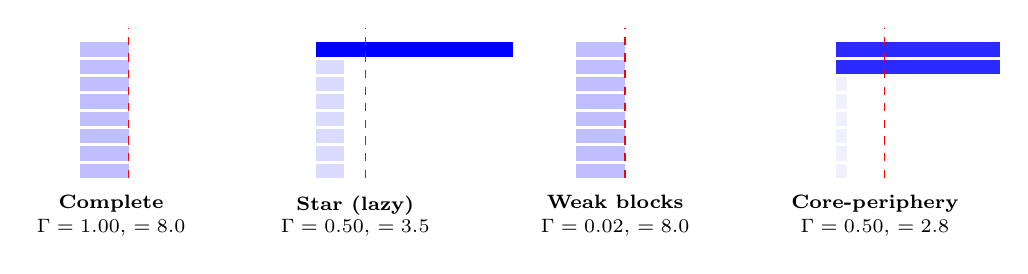
\begin{tikzpicture}[scale=1]
%% Complete: flat bars (pi_i = 0.125)
\begin{scope}
\foreach \k in {1,...,8} {
  \fill[blue!25] (0, {(8-\k)*0.22}) rectangle ({0.125*5}, {(8-\k)*0.22+0.18});
}
\draw[red, dashed, thin] ({0.125*5}, 0) -- ({0.125*5}, 1.9);
\node[below, font=\scriptsize\bfseries] at (0.4, -0.1) {Complete};
\node[below, font=\scriptsize] at (0.4, -0.4) {$\Gamma = 1.00$, $\Neff = 8.0$};
\end{scope}

%% Star (lazy): hub 0.500, spokes 0.071
\begin{scope}[xshift=3.0cm]
\fill[blue!100] (0, {7*0.22}) rectangle ({0.500*5}, {7*0.22+0.18});
\foreach \k in {1,...,7} {
  \fill[blue!14] (0, {(\k-1)*0.22}) rectangle ({0.071*5}, {(\k-1)*0.22+0.18});
}
\draw[red, dashed, thin] ({0.125*5}, 0) -- ({0.125*5}, 1.9);
\node[below, font=\scriptsize\bfseries] at (0.5, -0.1) {Star (lazy)};
\node[below, font=\scriptsize] at (0.5, -0.4) {$\Gamma = 0.50$, $\Neff = 3.5$};
\end{scope}

%% Weak blocks (doubly stochastic): flat
\begin{scope}[xshift=6.3cm]
\foreach \k in {1,...,8} {
  \fill[blue!25] (0, {(8-\k)*0.22}) rectangle ({0.125*5}, {(8-\k)*0.22+0.18});
}
\draw[red, dashed, thin] ({0.125*5}, 0) -- ({0.125*5}, 1.9);
\node[below, font=\scriptsize\bfseries] at (0.5, -0.1) {Weak blocks};
\node[below, font=\scriptsize] at (0.5, -0.4) {$\Gamma = 0.02$, $\Neff = 8.0$};
\end{scope}

%% Core-periphery: core 0.417 (x2), periphery 0.028 (x6)
\begin{scope}[xshift=9.6cm]
\foreach \k/\val/\bp in {1/0.417/83,2/0.417/83,3/0.028/6,4/0.028/6,5/0.028/6,6/0.028/6,7/0.028/6,8/0.028/6} {
  \fill[blue!\bp] (0, {(8-\k)*0.22}) rectangle ({\val*5}, {(8-\k)*0.22+0.18});
}
\draw[red, dashed, thin] ({0.125*5}, 0) -- ({0.125*5}, 1.9);
\node[below, font=\scriptsize\bfseries] at (0.5, -0.1) {Core-periphery};
\node[below, font=\scriptsize] at (0.5, -0.4) {$\Gamma = 0.50$, $\Neff = 2.8$};
\end{scope}
\end{tikzpicture}
\end{center}
\vspace{-0.5em}
\small Power distributions ($\boldsymbol{\pi}$) for four of the constructions of Example~\ref{ch06:ex:gap}, at $N = 8$ (bar length $\propto \pi_i$, shade $= 200\pi_i$). Dashed red line: $1/N = 0.125$ (equal power). Complete and weak blocks are both perfectly flat, although their spectral gaps are 1.00 and 0.02. Star and core-periphery have the same gap (0.50) but different concentration. The shape of $\boldsymbol{\pi}$ is read from $\Neff$; $\Gamma$ reports how fast the network mixes, not how power is distributed.
\end{vizpanel}

\subsection{The Spectral Gap as Development Diagnostic}

\begin{prebisch}[Two coordinates of the global economy]
Combining the insights from Chapters~3 and~5, the global production share matrix $W^P_{\text{global}}$ has to be read on two coordinates. Its spectral gap measures how well integrated the global economy is: whether shocks and demand mix quickly across all regions, or stay trapped in weakly coupled blocks. Its Perron vector, summarized by $\Neff$, measures how concentrated structural power is.

Prebisch's center--periphery argument is about the second coordinate. The periphery depends on the center ($W^P_{\text{periphery, center}}$ large) while the center barely depends on the periphery ($W^P_{\text{center, periphery}} \approx 0$). That asymmetry concentrates $\boldsymbol{\pi}$ on the center (the core-periphery row of Example~\ref{ch06:ex:gap}: $\Neff = 2.85$ out of 10). It need not lower $\Gamma$ at all --- in that example $\Gamma = 0.5$, and if every country imported from the same core the matrix would be close to rank one, with $\Gamma$ close to 1. A world can be tightly integrated and highly unequal in power at the same time.

Domestic structural heterogeneity (Chapter~3) is, by contrast, about the first coordinate: weak links between the modern and traditional blocks make $\Gamma$ of Bolivia's domestic $W^P$ small (Proposition~\ref{ch06:prop:block_power}). Epistemic dependence (Chapter~5) is about the second: the Perron vector of the global $W^I$. The periphery's double trap is a statement on both coordinates, and the two have to be measured separately.
\end{prebisch}


%% =====================================================================
\section{Power in Practice}
\label{ch06:sec:practice}
%% =====================================================================

\subsection{Where Does Power Come From?}

The Perron eigenvector gives us a precise answer. From equation~\eqref{ch06:eq:perron_component}:
\begin{equation}
\pi_i = \frac{1}{\rho} \sum_{j=1}^N \pi_j W_{ji}.
\end{equation}

Your power is the weighted sum of the power of agents who depend on you, where the weights are how much they depend on you. This generates three \textit{sources} of structural power:

\textbf{1. Being needed (production power).} If many agents use your output as an input ($W^P_{ji}$ large for many $j$), you have production power. Saudi Arabia has production power in the global oil network. TSMC has production power in the semiconductor network.

\textbf{2. Being cared about (social power).} If powerful agents care about your wellbeing ($W^U_{ji}$ large for powerful $j$), you have social power. The president's spouse has social power. A patron's favored client has social power.

\textbf{3. Being listened to (epistemic power).} If powerful agents pay attention to your signals ($W^I_{ji}$ large for powerful $j$), you have epistemic power. The Federal Reserve chair has epistemic power. A TikTok influencer has epistemic power.

\subsection{Power vs.\ Wealth}

Power $(\boldsymbol{\pi})$ and wealth $(\mathbf{w})$ are not the same thing.

Wealth is what you have --- your endowment $\omega_i$, your capital $K_i$, your income $Y_i$. Wealth can be redistributed by transfers: tax the rich, give to the poor, and $\mathbf{w}$ changes.

Power is where you sit --- your position in $W$. Holding $W$ fixed, a transfer changes $\boldsymbol{\omega}$ but not $\boldsymbol{\pi}$: the Perron eigenvector is a property of the matrix, not of the endowment vector. (If $W$ itself responds to the allocation --- the feedback studied from Chapter~7 on --- transfers can move $\boldsymbol{\pi}$ indirectly.)

\begin{example}[A Rich Farmer and a Poor Minister]\label{ch06:ex:rich_poor}
Suppose agent 1 is a wealthy farmer ($w_1 = 100$) and agent 2 is a poor government minister ($w_2 = 10$). In a $2 \times 2$ economy with:
\begin{equation}
W = \begin{pmatrix} 0.8 & 0.2 \\ 0.9 & 0.1 \end{pmatrix},
\end{equation}
the farmer depends on himself ($W_{11} = 0.8$) and barely on the minister ($W_{12} = 0.2$). But the minister depends heavily on the farmer ($W_{21} = 0.9$) --- because agricultural output feeds the government's tax base.

The rows sum to one ($0.8 + 0.2 = 0.9 + 0.1 = 1$), so $W$ is row-stochastic and $\rho = 1$. The left Perron eigenvector solves $\boldsymbol{\pi}' W = \boldsymbol{\pi}'$. From the first column: $0.8\pi_1 + 0.9\pi_2 = \pi_1$, so $\pi_2/\pi_1 = 0.2/0.9 = 2/9$. With $\pi_1 + \pi_2 = 1$: $\pi_1 = 9/11 \approx 0.818$, $\pi_2 = 2/11 \approx 0.182$.

The farmer has 82\% of the structural power despite the minister having the political title. Why? Because the minister depends on the farmer (for tax revenue) more than the farmer depends on the minister (for governance). The dependency is asymmetric, and asymmetry is power.

The farmer is rich AND powerful. The minister is poor AND less powerful. This is a structurally stable configuration: power and wealth reinforce each other. Chapter~13 will show that such configurations are fixed points of the structural reproduction process.
\end{example}


%% =====================================================================
\section{Summary}
\label{ch06:sec:summary}
%% =====================================================================

\begin{enumerate}
\item \textbf{Four centrality measures} capture different aspects of network importance: degree counts direct connections; Katz counts all paths, discounted; Bonacich is Katz rescaled, with an interpretable sign; and the eigenvector is recursive power. Eigenvector centrality is the parameter-free limit of the Katz family.

\item \textbf{The Perron-Frobenius theorem} guarantees that $\boldsymbol{\pi}$ exists, is unique, and is positive for any irreducible (strongly connected) nonnegative matrix; strict dominance of the Perron root, and convergence of $W^t$, need primitivity (aperiodicity as well).

\item \textbf{Power is equal if and only if a row-stochastic $W$ is doubly stochastic.} This is a distributional statement. The First Welfare Theorem holds for the Walrasian $W^{\text{mkt}} = \ones\mathbf{s}'$ with any wealth shares $\mathbf{s}$; efficiency fails through externalities ($W^U \neq 0$), not through unequal $\boldsymbol{\pi}$.

\item \textbf{Two coordinates, not one.} The spectral gap $\Gamma = 1 - |\lambda_2|$ measures integration (mixing speed, fragmentation); the concentration of power is measured by $\Neff = 1/\sum\pi_i^2$, $\Var(\boldsymbol{\pi})$ or the power Gini. The two are independent (Proposition~\ref{ch06:prop:gap-power-independent}).

\item \textbf{Power comes from position}, not endowment. Holding $W$ fixed, transfers change $\boldsymbol{\omega}$ but not $\boldsymbol{\pi}$; structural policy changes $W$ and therefore $\boldsymbol{\pi}$, with sensitivities given by Lemma~\ref{ch06:lem:perturbation}.
\end{enumerate}


%% =====================================================================
\section{Exercises}
\label{ch06:sec:exercises}
%% =====================================================================

\begin{enumerate}[label=\textbf{6.\arabic*}, leftmargin=3em]

\item \textbf{Computing centralities.} For the five-agent economy~\eqref{ch06:eq:W5}:
\begin{enumerate}
\item Compute all four centrality measures: degree, Katz with $\delta = 0.5$, Bonacich with $\beta = 0.3$, and eigenvector. Use Python.
\item Do they agree on the ranking? Where do they disagree?
\item Now double $W_{31}$ (Agent~3 depends more on Agent~1), taking the extra $0.1$ from $W_{33}$ so the row still sums to one. Recompute the eigenvector centrality. Does Agent~1's power rise? By how much? (Check your answer against Proposition~\ref{ch06:prop:monotone}.)
\end{enumerate}

\item \textbf{Doubly stochastic or not.} Classify each matrix as doubly stochastic (equal power) or not (asymmetric power), and for those that are not, find the Perron eigenvector:
\begin{enumerate}
\item $W = \frac{1}{3}\begin{pmatrix} 1 & 1 & 1 \\ 1 & 1 & 1 \\ 1 & 1 & 1 \end{pmatrix}$
\item $W = \begin{pmatrix} 0.5 & 0.5 \\ 0.8 & 0.2 \end{pmatrix}$
\item $W = \begin{pmatrix} 0.5 & 0.5 & 0 \\ 0 & 0.5 & 0.5 \\ 0.5 & 0 & 0.5 \end{pmatrix}$ (compare with (a): same $\boldsymbol{\pi}$? same $\Gamma$?)
\item $W = \begin{pmatrix} 0.4 & 0.3 & 0.3 \\ 0.3 & 0.4 & 0.3 \\ 0.3 & 0.3 & 0.4 \end{pmatrix}$
\end{enumerate}

\item \textbf{The spectral gap and convergence.} For each topology (complete, lazy star, lazy ring, weak blocks with $\varepsilon = 0.01$), built as in Example~\ref{ch06:ex:gap} with $N = 8$:
\begin{enumerate}
\item Compute $\Gamma$ and $\Neff$. Then compute $\Gamma$ for the ring and the star \textit{without} self-loops, and explain why it is zero.
\item Starting from $\mathbf{b}^{(0)} = (1, 0, 0, 0, 0, 0, 0, 0)'$, iterate $\mathbf{b}^{(t+1)} = W\mathbf{b}^{(t)}$ for $t = 1, \ldots, 50$. Plot $\|\mathbf{b}^{(t)} - \boldsymbol{\pi}'\mathbf{b}^{(0)}\ones\|$ (distance from consensus) against $t$.
\item Verify that the convergence rate matches $|\lambda_2|^t$.
\end{enumerate}

\item \textbf{Bonacich with negative $\beta$.} For a buyer-seller network:
\begin{equation}
W = \begin{pmatrix} 0 & 0 & 0.5 & 0.5 \\ 0 & 0 & 0.5 & 0.5 \\ 0.5 & 0.5 & 0 & 0 \\ 0.5 & 0.5 & 0 & 0 \end{pmatrix}.
\end{equation}
\begin{enumerate}
\item Compute Bonacich centrality with $\beta = 0.3$ (cooperation) and $\beta = -0.3$ (bargaining).
\item Under bargaining ($\beta < 0$), which agents have higher centrality? Why?
\item Relate to Manea's (2011) bargaining result: in symmetric bipartite networks, all agents have equal bargaining power. Does the eigenvector centrality confirm this? Compute $\Gamma$ for this $W$ and explain the value (the network is bipartite).
\end{enumerate}

\item \textbf{Power iteration by hand.} For $W = \begin{pmatrix} 0.6 & 0.4 \\ 0.2 & 0.8 \end{pmatrix}$:
\begin{enumerate}
\item Start with $\mathbf{v}^{(0)} = (1, 1)$. Compute $\mathbf{v}^{(1)} = W'\mathbf{v}^{(0)}$, normalize. Repeat for $t = 2, 3, 4, 5$.
\item At what iteration does $\mathbf{v}^{(t)}$ converge to two decimal places?
\item Compute the exact Perron eigenvector algebraically (solve $\boldsymbol{\pi}'W = \boldsymbol{\pi}'$).
\item Compare with the iterative result. Compute $\Gamma$ and verify the convergence rate.
\end{enumerate}

\item \textbf{Structural power vs.\ formal power.} An economy has 4 agents: President, General, Businesswoman, Farmer. Construct a plausible $4 \times 4$ weight matrix where the Farmer has the highest eigenvector centrality despite having the lowest formal rank. (Hint: make everyone's food supply depend on the Farmer, directly or indirectly.) Compute $\boldsymbol{\pi}$ and verify.

\item \textbf{Bolivia's power structure.} Using the Bolivia three-sector model from Chapter~3 ($W^P$ with Gas, Manufacturing, Traditional):
\begin{enumerate}
\item Compute the left Perron eigenvector. Which sector has the most structural power?
\item Now suppose gas revenues are redistributed to the traditional sector (a transfer). Does $\boldsymbol{\pi}$ change? Why or why not?
\item Now suppose a gas-to-fertilizer plant is built, adding a link from Gas to Traditional ($W^P_{\text{Trad, Gas}}$ increases from 0.02 to 0.15, with the Traditional row's own entry reduced by the same amount so the row still sums to one). Recompute $\boldsymbol{\pi}$. How does the traditional sector's power change?
\item Which policy --- the transfer or the plant --- changes the power structure?
\item \textit{Data.} Download a published input-output table (INE Bolivia's \textit{Matriz Insumo-Producto}, or a Latin American country in the OECD ICIO tables), aggregate it to three sectors, form the share matrix $W^P = D^{-1}A$, and compute $\boldsymbol{\pi}$, $\Neff$ and $\Gamma$. Compare with the stylized model.
\end{enumerate}

\end{enumerate}


%% =====================================================================
\newpage
\section*{Mathematical Appendices}
\addcontentsline{toc}{section}{Mathematical Appendices}
%% =====================================================================


\subsection*{Appendix 6A: Computing the Perron Eigenvector}
\addcontentsline{toc}{subsection}{Appendix 6A: Computing the Perron Eigenvector}
\label{ch06:app:computing}

\paragraph{Power iteration.} The simplest algorithm:
\begin{enumerate}
\item Start with $\mathbf{v}^{(0)} = \frac{1}{N}\ones$ (or any positive vector).
\item Iterate: $\tilde{\mathbf{v}}^{(t+1)} = W' \mathbf{v}^{(t)}$ (multiply by the transpose).
\item Normalize: $\mathbf{v}^{(t+1)} = \tilde{\mathbf{v}}^{(t+1)} / \|\tilde{\mathbf{v}}^{(t+1)}\|_1$.
\item Repeat until $\|\mathbf{v}^{(t+1)} - \mathbf{v}^{(t)}\|_\infty < \varepsilon$ (convergence tolerance).
\end{enumerate}

The spectral radius is estimated as $\rho \approx \|\tilde{\mathbf{v}}^{(t+1)}\|_1 / \|\mathbf{v}^{(t)}\|_1$ (the growth factor before normalization).

\paragraph{Convergence rate.} For primitive $W$ the error after $t$ iterations is $\|\mathbf{v}^{(t)} - \boldsymbol{\pi}\| = O(|\lambda_2/\rho|^t)$ (times a polynomial in $t$ if $\lambda_2$ is defective). For row-stochastic $W$ the rate is $|\lambda_2| = 1 - \Gamma$. For the complete graph ($\Gamma = 1$): convergence in one step. For a weakly coupled block graph ($\Gamma \approx 0.01$): each digit of accuracy requires $\ln 10/(-\ln 0.99) \approx 230$ iterations. For periodic $W$ ($\Gamma = 0$) plain power iteration does not converge; iterate the lazy matrix $\frac12(I+W)$, which has the same $\boldsymbol{\pi}$.

\paragraph{Python code.}
\begin{verbatim}
import numpy as np

def perron_eigenvector(W, tol=1e-10, maxiter=1000):
    """Left Perron eigenvector of W."""
    n = W.shape[0]
    v = np.ones(n) / n
    for _ in range(maxiter):
        v_new = W.T @ v
        v_new = v_new / v_new.sum()
        if np.max(np.abs(v_new - v)) < tol:
            return v_new
        v = v_new
    return v

def spectral_gap(W):
    """Gamma = 1 - |lambda_2| for row-stochastic W."""
    eigenvalues = np.sort(np.abs(np.linalg.eigvals(W)))[::-1]
    return 1 - eigenvalues[1]

def n_eff(pi):
    """Effective number of agents, 1 / sum pi_i^2."""
    return 1 / np.sum(pi ** 2)
\end{verbatim}
All numbers in this chapter are reproduced by \texttt{code/ch06.py}.

\paragraph{Computational complexity.} Each iteration of power iteration requires one matrix-vector multiplication: $O(N^2)$ for a dense matrix, $O(\text{nnz})$ for a sparse matrix (where $\text{nnz}$ is the number of nonzero entries). For most economic networks (sparse, $\text{nnz} \ll N^2$), this is efficient even for $N$ in the millions.


\subsection*{Appendix 6B: Proof of Perron-Frobenius (Positive Case)}
\addcontentsline{toc}{subsection}{Appendix 6B: Proof of Perron-Frobenius (Positive Case)}
\label{ch06:app:PF_proof}

We prove Theorem~\ref{ch06:thm:PF} for the case $W > 0$ (all entries strictly positive). The irreducible case requires additional machinery (see Horn and Johnson, 2012, Chapter~8).

\paragraph{Setup.} Let $W > 0$ be $N \times N$ with all entries strictly positive. Define the positive cone $\mathcal{K} = \{\x \in \R^N : x_i > 0 \text{ for all } i\}$ and the simplex $\Delta = \{\x \in \mathcal{K} : \|\x\|_1 = 1\}$.

\paragraph{Step 1: $W$ maps the positive cone to itself.} Since $W > 0$ and $\x > 0$, the product $W\x$ has all positive entries: $(W\x)_i = \sum_j W_{ij}x_j > 0$.

\paragraph{Step 2: Hilbert projective metric.} For $\x, \y \in \mathcal{K}$, define:
\begin{equation}
M(\x/\y) = \max_i \frac{x_i}{y_i}, \qquad m(\x/\y) = \min_i \frac{x_i}{y_i}, \qquad d_H(\x, \y) = \ln \frac{M(\x/\y)}{m(\x/\y)}.
\end{equation}
This is a pseudo-metric on the positive cone ($d_H(\x, \y) = 0$ iff $\x = c\y$ for some $c > 0$). Restricted to the open simplex $\Delta$ (one representative per ray) it is a metric, and $(\Delta, d_H)$ is complete.

\paragraph{Step 3: Birkhoff's contraction.} For $W > 0$, Birkhoff's theorem gives $d_H(W\x, W\y) \leq \tau(W)\, d_H(\x, \y)$ with $\tau(W) = \frac{1 - \sqrt{\phi(W)}}{1 + \sqrt{\phi(W)}}$, where $\phi(W) = \min_{i,j,k,l} \frac{W_{ik}W_{jl}}{W_{jk}W_{il}} > 0$. (The cruder ratio $(\min_{ij} W_{ij}/\max_{ij} W_{ij})^2$ is a lower bound for $\phi(W)$, so it also yields a valid $\tau < 1$.) Since $\phi(W) > 0$, $\tau(W) < 1$: the map $\x \mapsto W\x$ is a strict contraction in the Hilbert metric.

\paragraph{Step 4: Existence and uniqueness.} The normalized map $T(\x) = W\x/\|W\x\|_1$ sends $\Delta$ into itself and satisfies $d_H(T\x, T\y) = d_H(W\x, W\y)$, so it is a contraction on the complete metric space $(\Delta, d_H)$. By the Banach fixed-point theorem, $T$ has a unique fixed point $\mathbf{v}^* \in \Delta$. This satisfies $W\mathbf{v}^* = \rho \mathbf{v}^*$ where $\rho = \|W\mathbf{v}^*\|_1 > 0$. Uniqueness in $\Delta$ means there is no other positive eigenvector, up to scale.

\paragraph{Step 5: Positivity and the left eigenvector.} $\mathbf{v}^* \in \Delta$, so $\mathbf{v}^* > 0$. Applying Steps 1--4 to $W' > 0$ gives a unique $\boldsymbol{\pi} > 0$ in $\Delta$ with $W'\boldsymbol{\pi} = \rho'\boldsymbol{\pi}$. Since $\rho'\boldsymbol{\pi}'\mathbf{v}^* = \boldsymbol{\pi}'W\mathbf{v}^* = \rho\boldsymbol{\pi}'\mathbf{v}^*$ and $\boldsymbol{\pi}'\mathbf{v}^* > 0$, $\rho' = \rho$: $\boldsymbol{\pi}'W = \rho\boldsymbol{\pi}'$.

\paragraph{Step 6: Dominance.} Let $W\mathbf{u} = \lambda\mathbf{u}$ with $\mathbf{u} \in \mathbb{C}^N \setminus \{0\}$ and $|\lambda| = \rho$. Entrywise, $\rho|\mathbf{u}| = |W\mathbf{u}| \leq W|\mathbf{u}|$. Multiply the nonnegative vector $W|\mathbf{u}| - \rho|\mathbf{u}|$ by $\boldsymbol{\pi}' > 0$: $\boldsymbol{\pi}'W|\mathbf{u}| - \rho\boldsymbol{\pi}'|\mathbf{u}| = 0$, so $W|\mathbf{u}| = \rho|\mathbf{u}|$. By Step 4, $|\mathbf{u}| = c\,\mathbf{v}^*$ with $c > 0$. Equality in $|\sum_j W_{ij}u_j| = \sum_j W_{ij}|u_j|$ with all $W_{ij} > 0$ forces all $u_j$ to share one argument $\theta$: $\mathbf{u} = e^{i\theta}c\,\mathbf{v}^*$. Then $\lambda\mathbf{u} = W\mathbf{u} = \rho\mathbf{u}$, so $\lambda = \rho$, and its eigenspace is spanned by $\mathbf{v}^*$. Hence every other eigenvalue has $|\lambda_k| < \rho$.

\paragraph{Step 7: Algebraic simplicity.} If $\rho$ were not algebraically simple, there would be $\mathbf{w}$ with $(W - \rho I)\mathbf{w} = \mathbf{v}^*$. Premultiplying by $\boldsymbol{\pi}'$ gives $0 = \boldsymbol{\pi}'\mathbf{v}^* > 0$, a contradiction.

This completes the proof for the positive case. For an irreducible and aperiodic $W$, some power $W^m$ is positive, and applying the result to $W^m$ yields items (1)--(4) for $W$; for irreducible periodic $W$ only (2)--(4) survive (Horn and Johnson, 2012, Chapter~8). $\square$

\subsection*{Appendix 6C: Perturbation of the Perron Vector and of the Spectral Gap}
\addcontentsline{toc}{subsection}{Appendix 6C: Perturbation of the Perron Vector and of the Spectral Gap}
\label{ch06:app:perturbation}

This lemma is the single sensitivity result used throughout the book (Chapters~7, 8, 13, 14, 15, 23 and~24).

\begin{lemma}[Perturbation Lemma]\label{ch06:lem:perturbation}
Let $W$ be irreducible and row-stochastic with Perron vector $\boldsymbol{\pi}$. Let $E$ satisfy $E\ones = \mathbf{0}$ and $E_{ij} \geq 0$ wherever $W_{ij} = 0$, so that $W(t) = W + tE$ is row-stochastic, nonnegative and irreducible for small $t \geq 0$.
\begin{enumerate}
\item \textbf{Perron vector.} With the fundamental matrix $Z := (I - W + \ones\boldsymbol{\pi}')^{-1}$,
\begin{equation}\label{ch06:eq:dpi}
\frac{d\boldsymbol{\pi}'}{dt}\Big|_{t=0} = \boldsymbol{\pi}'EZ .
\end{equation}
If $W$ is diagonalizable with right eigenvectors $\mathbf{v}_k$ and left eigenvectors $\mathbf{u}_k'$ normalized biorthogonally ($\mathbf{u}_k'\mathbf{v}_l = \delta_{kl}$, $\mathbf{v}_1 = \ones$, $\mathbf{u}_1 = \boldsymbol{\pi}$), equivalently
\begin{equation}\label{ch06:eq:dpi_eig}
\frac{d\boldsymbol{\pi}'}{dt} = \sum_{k \geq 2} \frac{\boldsymbol{\pi}'E\mathbf{v}_k}{1 - \lambda_k}\,\mathbf{u}_k' .
\end{equation}
\item \textbf{Eigenvalues.} If $\lambda$ is a simple eigenvalue of $W$ with right vector $\mathbf{v}$, left vector $\mathbf{u}$ and $\mathbf{u}'\mathbf{v} = 1$, then $d\lambda/dt = \mathbf{u}'E\mathbf{v}$ and, for $\lambda \neq 0$,
\begin{equation}\label{ch06:eq:dabs}
\frac{d|\lambda|}{dt} = \frac{\operatorname{Re}\bigl(\bar{\lambda}\,\mathbf{u}'E\mathbf{v}\bigr)}{|\lambda|} .
\end{equation}
Hence $\Gamma = 1 - |\lambda_2|$ is differentiable along $E$ whenever $\lambda_2$ is simple and no eigenvalue other than $\lambda_2$ and its conjugate has modulus $|\lambda_2|$, with $d\Gamma/dt = -d|\lambda_2|/dt$.
\end{enumerate}
\end{lemma}

\begin{proof}
\textit{(1)} $\boldsymbol{\pi}(t)$ is the normalized left eigenvector of the simple eigenvalue $1$ of $W(t)$, hence differentiable in $t$. Differentiating $\boldsymbol{\pi}(t)'W(t) = \boldsymbol{\pi}(t)'$ and $\boldsymbol{\pi}(t)'\ones = 1$ at $t = 0$ gives $\dot{\boldsymbol{\pi}}'(I - W) = \boldsymbol{\pi}'E$ and $\dot{\boldsymbol{\pi}}'\ones = 0$. The second identity gives $\dot{\boldsymbol{\pi}}'\ones\boldsymbol{\pi}' = 0$, so $\dot{\boldsymbol{\pi}}'(I - W + \ones\boldsymbol{\pi}') = \boldsymbol{\pi}'E$. The matrix $I - W + \ones\boldsymbol{\pi}'$ is invertible: it maps $\ones$ to $\ones$, and on the $W$-invariant complement $\{\x : \boldsymbol{\pi}'\x = 0\}$ of $\operatorname{span}(\ones)$ it acts as $I - W$, whose eigenvalues there, $1 - \lambda_k$ ($k \geq 2$), are nonzero because the eigenvalue $1$ is simple. This gives~\eqref{ch06:eq:dpi}, with no diagonalizability needed. In the diagonalizable case $Z = \ones\boldsymbol{\pi}' + \sum_{k \geq 2}(1-\lambda_k)^{-1}\mathbf{v}_k\mathbf{u}_k'$, and $\boldsymbol{\pi}'E\ones = 0$ gives~\eqref{ch06:eq:dpi_eig}.

\textit{(2)} Differentiating $W(t)\mathbf{v}(t) = \lambda(t)\mathbf{v}(t)$ gives $E\mathbf{v} + W\dot{\mathbf{v}} = \dot\lambda\mathbf{v} + \lambda\dot{\mathbf{v}}$; premultiplying by $\mathbf{u}'$ and using $\mathbf{u}'W = \lambda\mathbf{u}'$ and $\mathbf{u}'\mathbf{v} = 1$ gives $\dot\lambda = \mathbf{u}'E\mathbf{v}$. Finally $|\lambda|^2 = \lambda\bar\lambda$, so $2|\lambda|\,\tfrac{d|\lambda|}{dt} = 2\operatorname{Re}(\bar\lambda\dot\lambda)$.
\end{proof}

\paragraph{Three consequences.}
\begin{enumerate}
\item \textbf{A common error.} A formula of the form $\sum_{k\geq2}(1-\lambda_k)^{-1}\mathbf{u}_k(\mathbf{u}_k'E\mathbf{v}_1)$ is identically zero, because $E\mathbf{v}_1 = E\ones = \mathbf{0}$ for every row-sum-preserving perturbation. The correct projection is onto $\boldsymbol{\pi}'E$, as in~\eqref{ch06:eq:dpi_eig}. Similarly, $\operatorname{sign}(\lambda)\,d\lambda$ is not the derivative of $|\lambda|$ when $\lambda$ is complex; use~\eqref{ch06:eq:dabs}.

\item \textbf{When is power cheap to move?} By~\eqref{ch06:eq:dpi_eig}, $\boldsymbol{\pi}$ is most sensitive when some $\lambda_k$ is close to $+1$, i.e.\ when $1 - \lambda_2$ is small (weakly coupled blocks). Eigenvalues near $-1$ (periodicity) give $1 - \lambda_k \approx 2$ and create no sensitivity. So the cost of moving power by a given amount --- through manipulation (Chapter~8) or escape (Chapter~7) --- scales \textit{with} $1 - \lambda_2$: it is smallest in fragmented networks, not largest.

\item \textbf{Where to add links to raise $\Gamma$.} Moving weight $t$ in row $j$ from $k$ to $i$ ($E = \mathbf{e}_j(\mathbf{e}_i - \mathbf{e}_k)'$) changes $\lambda_2$ by $t\,u_{2j}(v_{2i} - v_{2k})$, to first order. The largest entries of $|\mathbf{u}_2|$ and $|\mathbf{v}_2|$ lie deep \textit{inside} the blocks, not on the bridge nodes. Example (\texttt{code/ch06.py}): two five-agent path-like blocks joined by a weak bridge, $\Gamma = 0.025$; moving self-weight into a link between the two block cores raises $\Gamma$ at rate $0.182$, while the same move between the two bridge nodes raises it at rate $0.109$. Raising integration means connecting the cores of the blocks, not reinforcing the existing bridge.
\end{enumerate}


%% =====================================================================
\subsection*{Structuralist Case Study: Prebisch's \textit{Capitalismo Perif\'{e}rico} and the Perron Eigenvector}
\addcontentsline{toc}{subsection}{Structuralist Case Study: Prebisch (1981)}
%% =====================================================================

In 1981, at the age of eighty, Ra\'{u}l Prebisch published \textit{Capitalismo Perif\'{e}rico: Crisis y Transformaci\'{o}n} (M\'{e}xico: Fondo de Cultura Econ\'{o}mica, 344~pp.) --- his final major work and, in many ways, his most theoretically ambitious. Where the 1949 manifesto diagnosed the center-periphery structure of international trade, \textit{Capitalismo Perif\'{e}rico} turned inward, analyzing the \textbf{power structure within peripheral capitalism} and the mechanisms through which the economic surplus is appropriated by those at the top of the social hierarchy.

The book's argument maps directly onto this chapter's formal framework.

% TODO-VERIFY: Prebisch's definition of the excedente in Capitalismo Periferico (FCE 1981; Part I) -- check against the text and add a page.
\textbf{Part 1: The surplus and its appropriation.} Prebisch's \textit{excedente} is, roughly, the part of the fruits of rising productivity that is not transferred to the labor force but retained by the owners of the means of production. In a capitalist economy, the surplus is not distributed by a planner; it is \textit{appropriated} through a power structure. The agents who appropriate the most surplus are not necessarily the most productive --- they are the ones with the strongest structural position. In this book's formalization (an interpretation, not Prebisch's own notation) the division of a surplus $\Phi$ follows the allocation rule of Chapter~7, $x_i = \Omega/N + (\pi_i - 1/N)\Phi$ (Proposition~\ref{ch07:prop:allocation-rule}): agents with $\pi_i > 1/N$ capture more than an equal share, regardless of their marginal product. Proposition~\ref{ch06:prop:equal_power} states the condition under which appropriation is equal: $W$ must be doubly stochastic. Prebisch's book can be read as an argument that peripheral $W$ is far from doubly stochastic.

\textbf{Part 2: Power is relational, not individual.} Prebisch explicitly rejected the neoclassical view that factor payments reflect marginal products. In peripheral capitalism, wages are held below marginal product not because of market imperfections (in the neoclassical sense) but because \textit{the power structure of the labor market favors employers}. The employer's structural position --- monopsony in thin labor markets, control over hiring and firing in the absence of unions, political connections that shape regulation --- gives her a Perron weight $\pi_{\text{employer}} \gg 1/N$. The worker's structural position --- limited outside options, geographic immobility, dependence on a single employer --- gives $\pi_{\text{worker}} \ll 1/N$. The wage is determined not by the intersection of supply and demand curves but by the bargaining equilibrium of Chapter~7, with weights from the Perron eigenvector of this chapter.

This is exactly equation~\eqref{ch06:eq:perron_component}: $\pi_i = \frac{1}{\rho}\sum_j \pi_j W_{ji}$. The worker's power is low because the powerful agents who ``point toward'' her (her employers) do not depend heavily on her individually ($W_{ji}$ small for any specific worker $j$). The employer's power is high because workers depend heavily on her ($W_{ij}$ large for many workers $i$). The recursion --- power comes from being depended upon by the powerful --- is the mathematical content of Prebisch's argument that ``power relations between social strata'' determine surplus appropriation.

\textbf{Part 3: The political economy of structural reproduction.} Prebisch argued that the power structure reproduces itself politically: those who appropriate the surplus use part of it to maintain the institutions (legal frameworks, education systems, media) that sustain their structural position. In the notation of Chapters~5 and~8: the powerful invest in $W^I$ (shaping information flows to justify the existing distribution) and in $W^P$ (maintaining production structures that keep their Perron weight high). How concentrated the resulting power is, is measured by $\Neff$ (Definition~\ref{ch06:def:neff}); the spectral gap does not measure it (Proposition~\ref{ch06:prop:gap-power-independent}). How hard the structure is to dislodge is a question about the sensitivity of $\boldsymbol{\pi}$ to changes in $W$ (Lemma~\ref{ch06:lem:perturbation}), taken up in Chapters~7 and~13.

\begin{center}
\begin{tabularx}{\textwidth}{LLL}
\toprule
\textbf{Prebisch's argument (1981)} & \textbf{Formal object} & \textbf{This chapter} \\
\midrule
Surplus appropriated by power & $\boldsymbol{\pi}(W)$ enters the allocation rule & Def.~\ref{ch06:def:eigenvector}; Prop.~\ref{ch07:prop:allocation-rule} \\
Power is relational, not individual & $\pi_i = \frac{1}{\rho}\sum_j \pi_j W_{ji}$ (recursive) & Eq.~\eqref{ch06:eq:perron_component} \\
Equal appropriation iff balanced dependence & $\boldsymbol{\pi} = \frac{1}{N}\ones$ iff $W$ doubly stochastic & Prop.~\ref{ch06:prop:equal_power} \\
Power concentrates in hubs & Star: $\pi_h = a/(a+1-s)$ & Prop.~\ref{ch06:prop:star_power} \\
Concentration of power & $\Neff$, $\Var(\boldsymbol{\pi})$; independent of $\Gamma$ & Def.~\ref{ch06:def:neff}; Prop.~\ref{ch06:prop:gap-power-independent} \\
Power $\neq$ wealth & $\boldsymbol{\pi}$ is property of $W$, not $\boldsymbol{\omega}$ & Ex.~\ref{ch06:ex:rich_poor} \\
\bottomrule
\end{tabularx}
\end{center}

Prebisch was eighty when he wrote this. He had spent three decades building institutions (CEPAL, UNCTAD, ILPES) and two decades watching those institutions' prescriptions --- import substitution, regional integration, international commodity agreements --- partially succeed and partially fail. \textit{Capitalismo Perif\'{e}rico} was his attempt to explain why: the structural policies he had championed changed $W^P$ (the production network) but did not change the \textit{power structure} that determined who appropriated the gains. The Perron eigenvector shifted, but not enough, because the other networks ($W^U$, $W^I$) reproduced the old $\boldsymbol{\pi}$.

The Perron-Frobenius theorem guarantees that $\boldsymbol{\pi}$ exists and is unique for any strongly connected $W$. What Prebisch understood at eighty, without the theorem, is that $\boldsymbol{\pi}$ is the object that determines who gets what --- and that changing it requires changing all three networks, not just one.


%% =====================================================================
\subsection*{Further Reading}
\addcontentsline{toc}{subsection}{Further Reading}
%% =====================================================================

\textbf{The Perron-Frobenius theorem:} Horn and Johnson (2012), \textit{Matrix Analysis}, Chapter~8 --- the definitive treatment. Seneta (2006), \textit{Non-Negative Matrices and Markov Chains} --- for the probabilistic perspective. Meyer (2000), \textit{Matrix Analysis and Applied Linear Algebra}, Chapter~8 --- accessible.

\textbf{Centrality measures:} Bonacich (1987), ``Power and Centrality: A Family of Measures,'' \textit{American Journal of Sociology}. Ballester, Calv\'{o}-Armengol, and Zenou (2006), ``Who's Who in Networks,'' \textit{Econometrica}. Jackson (2008), \textit{Social and Economic Networks}, Chapter~2.

% TODO-VERIFY: venue of Golub (2025), "Eigenvalues in Microeconomics" (arXiv preprint? Notices of the AMS?).
\textbf{Spectral methods in economics:} Golub (2025), ``Eigenvalues in Microeconomics,'' \textit{Notices of the AMS}. Sargent and Stachurski (2024), \textit{Economic Networks}, Chapters~2--3. Acemoglu et al.\ (2012), ``Network Origins of Aggregate Fluctuations,'' for the ``influence vector'' $(\alpha/N)\ones'(I - (1-\alpha)W^P)^{-1}$ --- a Katz/Leontief object whose $\alpha \to 0$ limit is the Perron vector of the input-share matrix. Kemeny and Snell (1960), \textit{Finite Markov Chains}, and Meyer (1980), on the fundamental matrix used in Appendix~6C.

\textbf{Birkhoff's contraction:} Birkhoff (1957), ``Extensions of Jentzsch's Theorem,'' \textit{Transactions of the AMS}. Lemmens and Nussbaum (2012), \textit{Nonlinear Perron-Frobenius Theory} --- the modern reference.

\textbf{The structuralist tradition on power:} Prebisch (1981), \textit{Capitalismo Perif\'{e}rico: Crisis y Transformaci\'{o}n}, M\'{e}xico: FCE (the primary source for the case study above). Marini (1973), \textit{Dial\'{e}ctica de la dependencia} (superexploitation as $\pi_{\text{worker}} \ll 1/N$). Quijano (2000), ``Colonialidad del poder, eurocentrismo y Am\'{e}rica Latina'' (power as a multi-layer matrix).

\end{document}
